%October 2016, the 4th
\chapter{The Hamming Ball}

This Chapter introduces an important concept: the Hamming Ball.

\section{Hamming Space}

A \emph{space} is a set that has structure.
The set $\{0,1\}^{n}$ of binary strings of length $n$ can be made into a metric space.
To make it a metric space we have to define a metric (or distance) on it.

A metric over set $\X$ is a function $d: \X \times \X \rightarrow \Reals$ that has the following properties:
\begin{enumerate}
	\item it's greater than zero, \ie $d(x, y) \geq 0$ $\forall (x, y) \in \X \times \X$, with equality when its arguments are the same, \ie $d(x, y) = 0 \iff x = y$;
	\item it's symmetric, \ie $d(x, y) = d(y, x)$ $\forall (x, y) \in \X \times \X$;
	\item it satisfies the triangular inequality, \ie $d(x, y) \leq d(x, z) + d(z, y)$.
\end{enumerate}

For $\{0,1\}^{n}$ we define the \emph{Hamming metric}.
Consider two strings, $\str{x}, \str{y}  \in \{0, 1\}^n$.
Then their Hamming distance is defined as
\begin{equation}
	\hdist{\str{x}, \str{y}} = \abs{\{i : x_i \neq y_i\}}.
\end{equation}

The first two properties are trivial to see.
For the third property, consider three strings $\str{x}$, $\str{y}$, $\str{z} \in \{0,1\}^n$.
Let $D = \{i : x_i \neq y_i\}$ be the set of coordinates where they differ.
If $i \in D$, we have $x_{i} \neq y_{i}$.
What can happen to $z_{i}$?
Either $z_{i} \neq x_{i}$ or $z_{i} \neq y_{i}$.
If $i \not\in D$, $z_{i}$ is either equal to both $x_{i}$ and $y_{i}$, or it differs from both of them.
Thus, $\hdist{x_{i},y_{i}} \le \hdist{x_{i},z_{i}} + \hdist{z_{i},y_{i}}$ for all $i$.

Now, since the Hamming metric is additive, we have
\begin{align*}
	\hdist{\str{x},\str{y}} & =
	\sum_{i = 1}^n \hdist{x_i,y_i} \\
	& \le
	\sum_{i = 1}^n \hdist{x_i,z_i} +
	\sum_{i = 1}^n \hdist{z_i,y_i}
	=
	\hdist{\str{x},\str{z}} +
	\hdist{\str{z},\str{y}}
\end{align*}
which gives us the triangular inequality.

In general,  a distance is extended to a product space by summing the distances of the single components, as happens for the Hamming metric.

Consider a storage device that has $n$ cells, each containing either $0$ or $1$.
Suppose memory decays with time in some unknown way.
After some time the string memorised in the device will be different.
The Hamming distance tells us how much different.

If a string $\str{x}$ has been changed no more than $r$ times to become $\str{y}$, then $d_H(\str{x}, \str{y}) \leq r$.
We say that $\str{y}$ is in a \emph{Hamming Ball} of radius $r$ around $\str{x}$.

\begin{definition}[Hamming Ball]
	The Hamming Ball of radius $r$ and centre $\str{x}$ is the set
	\begin{equation}
		\hball{\str{x}}{r} = \{\str{y} : \hdist{\str{x},\str{y}} \leq r\}.
	\end{equation}
\end{definition}

\begin{obs}
	$r$ needs not to be an integer, but for $r \in \Reals$ it holds that
	\begin{equation*}
		\hball{\str{x}}{r} = \hball{\str{x}}{\floor{r}}.
	\end{equation*}
\end{obs}

Note that $\{0,1\}^{n}$ is a Hamming Ball of radius $n$, for any centre.

If you have a ball that is not the whole space, then the centre of this ball is unique.

What we can say about the size of a generic Hamming Ball $\hball{\str{x}}{r}$, with $r > 0$?
For the sake of simplicity, consider $\hball{\zero}{r}$, where $\zero$ is the string of all zeros.
Then the size of this Hamming Ball is
\begin{equation}\label{eq:volume}
	\abs{\hball{\zero}{r}} = \sum_{i = 0}^{\floor{r}} \binom{n}{i}
\end{equation}
\ie the number of ways in which we can flip to 1 up to $r$ bits.

\begin{definition}[Hamming weight]
	The Hamming weight of a string is its distance from $\zero$, \ie
	\begin{equation}
	\hweight{\str{x}} = \hdist{\zero,\str{x}}.
	\end{equation}
\end{definition}

If one subtracts $\hball{\str{x}}{r}$ to $\{0, 1\}^n$, then the result is also an Hamming ball.

To see this, consider a string $\str{y}$ that is not in $\hball{\zero}{r}$.
Then it must be that $\hweight{\str{y}} > r$.
What is its distance from the string of all ones, \ie $\hdist{\str{y},\str{1}}$?
One can see that $\hdist{\str{y},\str{1}} = n - \hweight{\str{y}}$, since $\hdist{\zero,\str{x}} + \hdist{\str{1},\str{x}} \ge \hdist{\str{0},\str{1}} = n$.
More in general we can bound the distance as $\hdist{\str{y},\str{1}} < n - r$, or $\hdist{\str{y},\str{1}} \le n - (r+1)$, which means that $\str{y}$ is in a Hamming Ball of radius $n - (r+1)$ with centre $\str{1}$.

From it we derive the following result:
\begin{equation*}
	\overline{\hball{\str{0}}{r}} = \{0,1\}^{n} \setminus \hball{\str{0}}{r} = \hball{\str{1}}{n - (r+1)}.
\end{equation*}
In other words the Hamming space can be partitioned into two Hamming balls.

If $n$ is odd, the Hamming space can be partitioned in the following way:
\begin{equation*}
	\{0, 1\}^n = \hball{\str{0}}{\floor{\frac{n}{2}}} \cup \hball{\str{1}}{\floor{\frac{n}{2}}}
\end{equation*}
The Hamming space cannot be partitioned into three balls.
In how many balls can $\{0, 1\}^n$ be partitioned?
It cannot be partitioned into $s$ balls with $3 \leq s \leq n + 1$ (this result has not been demonstrated).

\section{The Volume of the Hamming Ball}

We have seen that the volume of a generic Hamming ball is described by Equation \ref{eq:volume}.
We can use the Pascal triangle to get a feeling about the order of magnitude of the Hamming ball.
Consider the $n$th row in the triangle; since it is symmetric, if we split the row in half the sum of the terms of the first part is equal to the sum of the terms of the second part of the row.
The volume of the greatest ball is $\abs{\hball{\str{0}}{n}} = 2^n$.
Instead, the volume of the ball with radius $n/2$ (in the triangle's point of split) is $\frac{2^n}{2} = 2^n2^{-1} = 2^{n-1}$.
It follows, if $r \ge \frac{n}{2}$, that $2^{n-1} \le \abs{\hball{\str{0}}{r}} \le 2^n$.
Can we bound the volume for $r < \frac{n}{2}$?

\subsection{Entropy}
First we introduce the notion of \emph{entropy}.

\begin{definition}[Entropy]
Entropy is a function $h: [0, 1] \rightarrow [0, 1]$ defined as follows:
\begin{equation}
	h(t) = t\log_2\left(\frac{1}{t}\right) + (1 - t)\log_2\left(\frac{1}{1-t}\right).
\end{equation} 
\end{definition}

\begin{figure}[h!]
	\centering
	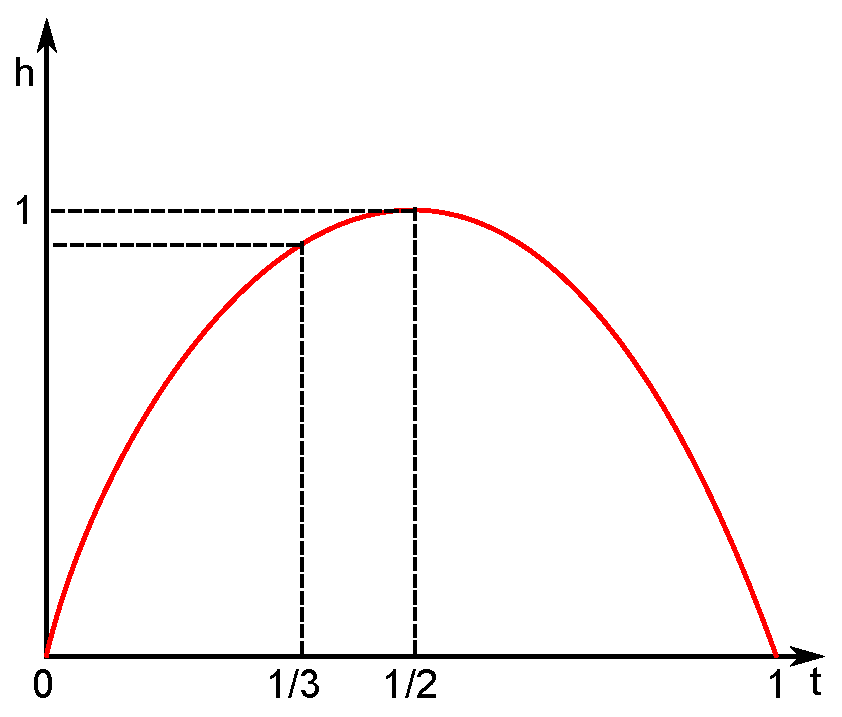
\includegraphics[width=0.5\linewidth]{pictures/ch01-i00.eps}
	\caption{The entropy function.}
\end{figure}

This function is not defined for the values $0$ and $1$.
However, we have limits defined on these points and they are both $0$.
So we artificially set $h(0) = 0$ and $h(1) = 0$.
It is better to think about a probability distribution $(t, 1 - t)$ and entropy is a number attached to it.
Entropy measures symmetry and with $t = \frac{1}{2}$ we have maximum chaos (the future outcomes are equally likely).

\subsection{Lower and Upper Bounds}

\begin{thm}[Upper bound of the volume of the Hamming Ball]
	The volue of the Hamming ball of radius $r$, for $r \leq \frac{n}{2}$, is
	\begin{equation*}
		\abs{\hball{\str{0}}{r}} \leq 2^{nh\left(\frac{r}{n}\right)}.
	\end{equation*}
\end{thm}

In order to prove this theorem an analogy is introduced.
Suppose there is a box with a number of chickens in it.
We want to count those animals without withdrawing all of them out of the box. What can be done is to take the lightest one and measure its weight $w$; then also the weight $W$ of the box is measured.
The number of the total chickens in the box can't be greater than $\frac{w}{W}$.

\begin{proof}
	In this proof we will use a similar technique.
	Consider $\{0, 1\}^n$.
	We ``sparkle'' a substance on the strings in the set; this substance looks like probability, but it doesn't matter.
	Define the weight of $1$ and $0$ as 
	\begin{equation*}
		P(1) = \frac{r}{n}, \quad P(0) = 1 - P(1).
	\end{equation*}
	Notice that is not an uniform distribution.
	Define the weight of a string as
	\begin{equation*}
		P^n\left(\str{x}\right) = \prod_{i = 1}^n P(x_i).
	\end{equation*}

	If $A \subseteq \{0, 1\}^n$, then the weight of the set $A$ is
	\begin{equation*}
		P^n(A) = \sum_{\str{x} \in A} P^n(\str{x}).
	\end{equation*}

	$P^n(\{0, 1\}^n)$ is the total weight of the substance sparkled on the strings and it is the probability distribution of binomial.
	For this reason one can claim that
	\begin{equation*}
		1
		=
		P^n (\{0, 1\}^n)
		\ge
		P^n \left(\hball{\str{0}}{r}\right)
		=
		\sum_{\str{x} \in \hball{\str{0}}{r}} P^n(\str{x}),
	\end{equation*}
	at this point we take out the lightest string and write
	\begin{equation*}
		\sum_{\str{x} \in \hball{\str{0}}{r}} P^n(\str{x})
		\ge
		\abs{\hball{\str{0}}{r}} \cdot \min_{\str{x} \in \hball{\str{0}}{r}} P^n(\str{x}).
	\end{equation*}

	Which are the lightest strings?
	Since we assumed that $r \leq \frac{n}{2}$ then
	\begin{equation*}
		r \le \frac{n}{2}
		\implies
		P(1) = \frac{r}{n} \le \frac{1}{2}
		\implies
		P(1) \le P(0).
	\end{equation*}
	It follows that the the lightest strings are the ones on the border of the ball, with $r$ $1$s. We now compute their weight.
	\begin{align*}
		\min_{\str{x} \in \hball{\str{0}}{r}} P^n(\str{x})
		& =
		\left[P(1)\right]^r \cdot \left[P(0)\right]^{n-r}
		\\
		& =
		\left(\frac{r}{n}\right)^r \left(1 - \frac{r}{n}\right)^{n-r}
		\\
		& =
		\left(\frac{r}{n}\right)^{n\frac{r}{n}} \left(1 - \frac{r}{n}\right)^{n\left(1 - \frac{r}{n}\right)}
		\\
		& =
		\left[\left(\frac{r}{n}\right)^{\frac{r}{n}} \left(1 - \frac{r}{n}\right)^{\left(1 - \frac{r}{n}\right)}\right]^n
		\\
		& =
		2^{n\log_2\left[\left(\frac{r}{n}\right)^{\frac{r}{n}}  \left(1 - \frac{r}{n}\right)^{\left(1 - \frac{r}{n}\right)}\right]}
		\\
		& =
		2^{n\left[\frac{r}{n}\log_2\frac{r}{n} + \left(1 - \frac{r}{n}\right)\log_2\left(1 - \frac{r}{n}\right)\right]}
		\\
		& =
		2^{-nh\left(\frac{r}{n}\right)}.
	\end{align*}

	So we have 
	\begin{equation*}
		1
		\geq
		\abs{\hball{\str{0}}{r}} \cdot \frac{1}{2^{nh\left(\frac{r}{n}\right)}}
		\implies
		\abs{\hball{\str{0}}{r}} \le 2^{n \, h\left(\frac{r}{n}\right)}.
	\end{equation*}
\end{proof}

\begin{thm}[Lower bound on the volume of the Hamming Ball]
	The volume of the Hamming ball of radius $r$, for $ r \leq \frac{n}{2}$, is
	\begin{equation*}
		\abs{\hball{\str{0}}{r}}
		\ge
		\frac{1}{n+1} \cdot 2^{n \, h\left(\frac{r}{n}\right)}.
	\end{equation*}
\end{thm}

\begin{proof}
	\begin{equation*}
		P(1) = \frac{r}{n},\quad P(0) = 1 - P(1),\quad P^n(\{0, 1\}^n) = 1.
	\end{equation*}
	Consider the set of all strings of length $n$ and partition it in the following way.
	\begin{equation*}
		T_q = \{\str{x}\ :\ \hweight{x} = q\},
	\end{equation*}
	obtaining $n +1$ classes. 
	We know that $\abs{T_q} = \binom{n}{q}$; we are not interested in how many strings are in that set, but what is the total weight.
	There is not symmetry in the weight of the partitions.
	In fact we can prove that
	\begin{equation*}
		\frac{P^n(T_q)}{P^n(T_r)} \le 1,\ \forall q.
	\end{equation*}
	In the formula above there are binomials we want to bound.
	In order to do that, we need the following observation.

	\begin{obs}
		\begin{equation*}
			\frac{k!}{l!} \le k^{k-l}.
		\end{equation*}
	\end{obs}

	\begin{proof}[Verification]
		If $k \ge l$:
			\begin{equation*}
				\frac{k!}{l!} = \frac{k(k-1) \cdots l(l -1) \cdots 1}{l(l -1) \cdots 1} \le k^{k-l}.
			\end{equation*}

		If $k < l$:
			\begin{equation*}
				\frac{k!}{l!} = \frac{k(k-1) \cdots 1}{l(l -1) \cdots k(k-1) \cdots 1} \le \left(\frac{1}{k+1}\right)^{l-k} < \left(\frac{1}{k}\right)^{l-k} = k^{k-l}.
			\end{equation*}
	\end{proof}

	Define $p = \frac{r}{n}$  so that we have a distribution $P(p, 1-p)$ that picks a set and concentrate the weight (probability) on it.
	We observe that the probability of each string in a class depends only on the number of $1$'s in it.
	So we can write
	\begin{align*}
		\frac{P^n(T_q)}{P^n(T_r)}
		& =
		\frac{p^q(1-p)^{n-q}\abs{T_q}}{p^r(1-p)^{n-r}\abs{T_r}}
		\\
		& =
		p^{q-r}(1-p)^{r-q} \frac{\frac{n!}{q!(n-q)!}}{\frac{n!}{r!(n-r)!}}
		\\
		& =
		p^{q-r}(1-p)^{r-q}\frac{r!}{q!}\frac{(n-r)!}{(n-q)!}
		\\
		& \le
		p^{q-r}(1-p)^{r-q}r^{r-q}(n-r)^{q-r}
		\\
		& =
		\tag{since $r = np$}
		p^{q-r}(1-p)^{r-q} (np)^{r-q}[n(1-p)]^{q-r}
		\\
		& =
		p^{q-r}(1-p)^{r-q}n^{r-q+q-r}p^{r-q}(1-p)^{q-r}
		\\
		& =
		p^{q-r + r-q}(1-p)^{r-q+q-r}
		=
		1.
	\end{align*}

	So we can write
	\begin{align*}
		1
		=
		P^n(\{0,1\}^n)
		& =
		P^n\left(\bigcup_{q=0}^nT_q\right)
		\\
		& =
		\sum_{q=0}^n P^n(T_q)
		\\
		& \le
		(n+1) \max_q P^n(T_q)
		\\
		& =
		(n+1) P^n(T_r)
		\\
		& =
		(n + 1) \abs{T_r} \cdot 2^{-n \, h \left(\frac{r}{n}\right)}
	\end{align*}

	Thus, we know that $\abs{T_r} \ge \frac{1}{n+1} 2^{n \, h(\frac{r}{n})}$, and since $T_r \subseteq \hball{\str{0}}{r}$ we have proved that $\abs{T_r} \le \abs{\hball{\str{0}}{r}}$.
\end{proof}

So this proof is important because the cardinality of the Hamming ball comes up in many contexts, such as error correction (a string that has been altered at most $r$ times is in a certain radius from the original string).

\section{Generalization to any finite alphabet}

Let $\X$ be the (usual) finite set that is an alphabet.
We are insterested in sequences of elements of $\X$, called \emph{strings} or \emph{words}.
So $\X^n, n \in \mathbb{N}$, is a set of words.
$\X^n$ can be partitioned by putting together those sequences that can be transformed one into the other by permutation, \ie sequences that have the same number of occurrences of elements in the alphabet.

\begin{definition}
	Let $a \in \X$ and $\str{x} \in \X^n$.
	We define the frequency of an alphabet symbol $a$ in a string $\str{x}$ in the following way:  
	\begin{equation*}
	N(a | \str{x}) = \abs{\{i\ :\ x_i = a\}}.
	\end{equation*}
	where $\str{x} = x_1 x_2 \ldots x_n$.
\end{definition}

One can think about ``normalized'' relative frequencies of symbols
\begin{equation*}
	\frac{1}{n} N(a|\str{x}).
\end{equation*}

Moreover the following holds:
\begin{equation*}
	\sum_{a \in \X} N(a|\str{x}) = n
	\implies \sum_{a\in \X} \frac{1}{n} N(a|\str{x}) = 1,
\end{equation*}
so from a string $\str{x}$ one can obtain a probability distribution over $\X$.
We define
\begin{equation*}
	P_{\str{x}} = \left\{ \frac{N(a|\str{x})}{n} : a \in \X \right\}
\end{equation*}
to be the \emph{type} of $\str{x}$.
There are just that many distributions for a number $n$; now fix a distribution $P|\X$.
$\exists \str{x} \in \X^n$ such that  $P_{\str{x}} = P$?
Yes, if and only if
\begin{equation*}
	P(a) = \dfrac{N(a | \str{x})}{n},\ \forall a \in \X.
\end{equation*}
Consider a product measure over $\X$; strings in the same partition have also the same ``length'' or measure.
Now, given $\X$ and $n$, how many distributions $P|\X$ are types in $\X^n$?
A rough upper bound is $(n + 1)^{\abs{\X}}$.
The last value is redundant, since the values sum up to $1$.
So we could do better with $(n + 1)^{\abs{\X} - 1}$.
We can partition $\X^n$ into sets of strings of the same type, $T_p$, with $P|\X$.
\begin{equation*}
	T_p = T_p^n = \{\str{x}\ :\ P_{\str{x}} = P\}.
\end{equation*}

\begin{definition}[Generalised Entropy]
	We introduce the \emph{generalized entropy} $H(P)$, defined as
	\begin{equation*}
		H(P) = -\sum_{a \in \X} P(a) \log_2 P(a).
	\end{equation*}
\end{definition}

\begin{thm} \label{thms:taupcard}
	If $T_p \neq \emptyset$ then $$\dfrac{1}{(n+1)^{|\X| -1}}2^{nH(P)}\leq |T_p| \leq 2^{nH(P)}$$
\end{thm}

\begin{proof}
	In order to prove the above theorem, we first define the product distribution $P|\X \rightarrow P^n|\X^n$ as 
	\begin{equation*}
		P^n(\str{x}) = \prod_{i = 1}^nP(x_i).
	\end{equation*}

	We can define it additively on subsets of $\X^n$.
	\begin{equation*}
		1 = P^n(\X^n) \ge P^n(T_p^n)
	\end{equation*}

	Now,
	\begin{align*}
		\forall \str{x} \in T_p^n . P^n(\str{x})
		& =
		\prod_{a \in \X} P(a)^{n P(a)}
		\\
		& =
		\prod_{a \in \X} 2^{n \, P(a)\log_2 P(a)} \tag{since it's independent of $\X$}
		\\
		& =
		2^{n \left[\sum_{a \in \X} P(a) \log_2 P(a) \right]}
		\\
		& =
		2^{-n \, H(p)}.
	\end{align*}

	So,
	\begin{equation*}
		1 = P^n(\X^n) \ge P^n(T^n_p) = \abs{T_p^n} \cdot 2^{-n \, H(p)}.
	\end{equation*}
\end{proof}

The lower bound proof is a straightforward generalization of what has been done in the binary case.
Entropy is greatest when the distribution is uniform.
Now, to prove the lower bound, consider
\begin{equation*}
	1
	=
	\sum_{P\ :\ T_p^n \neq \emptyset} P^n(T_p^n)
	\le
	(n+1)^{\abs{\X}-1} \max_{Q|\X} P^n(T_q^n).
\end{equation*}

\begin{obs}
	If $T^n_p \neq \emptyset$ then 
	\begin{equation*}
		\frac{P^n(T^n_q)}{P^n(T^n_p)} \le 1.
	\end{equation*}
	If a distribution is a type, it maximizes its (product) value on the strings of that type. 
\end{obs}

\begin{proof}
	We can suppose, without loss of generality, that $T^n_q \neq \emptyset$.
	\begin{align*}
		P^n(T_q^n)
		& =
		\prod_{a \in \X} P(a)^{n \, Q(a)} \abs{T_q^n}
		\\
		& \implies
		\\
		\frac{
			P^n(T_q^n)
		}{
			P^n(T_p^n)
		}
		& =
		\frac{
			\abs{T_q^n} \prod_{a \in \X} [P(a)]^{n Q(a)}
		}{
			\abs{T_p^n} \prod_{a \in \X} [P(a)]^{n P(a)}
		}
		\\
		& =
		\frac{
			\frac{n!}{\prod_{a\in\X} [nQ(a)]!} \prod_{a \in \X} [P(a)]^{n Q(a)}
		}{
			\frac{n!}{\prod_{a\in\X} [nP(a)]!} \prod_{a \in \X} [P(a)]^{n P(a)}
		}
		\\
		& =
		\prod_{a \in \X}
		\frac{[n \, P(a)]!}{[n \, Q(a)]!}
		\prod_{a \in \X}
		[P(a)]^{n \, (Q(a)-P(a))}
		\\
		& \le
		\prod_{a \in \X}
		[nP(a)]^{n \, (P(a)-Q(a))}
		\prod_{a \in \X}
		[P(a)]^{n \, (Q(a)-P(a))}
		\\
		& =
		n^{n \left[ \sum_{a \in \X} P(a) - Q(a) \right]}
		\frac{
			\prod_{a \in \X} [P(a)]^{n (P(a)-Q(a))}
		}{
			\prod_{a \in \X} [P(a)]^{n (P(a)-Q(a))}
		}
		\\
		& =
		n^{n \left[ \sum_{a \in \X} P(a) - \sum_{a \in \X} Q(a) \right]}
		\\
		& =
		n^{n[1-1]}
		=
		1.
	\end{align*}

	So we can write
	\begin{equation*}
		\max_{Q|\X} P^n(T_q^n)
		=
		\abs{T_p^n} \prod_{a \in \X} P(a)^{n \, P(a)}
		=
		\abs{T_p^n} \cdot 2^{-n \, H(P)}
	\end{equation*}
	and conclude that
	\begin{equation*}
		1
		\le
		(n+1)^{\abs{\X}-1} \abs{T_p^n} \cdot 2^{-n \, H(P)}
		\implies
		\frac{1}{(n+1)^{\abs{\X}-1}} \cdot 2^{n \, H(P)} \le \abs{T_p^n}.
	\end{equation*}
\end{proof}

